%% 
%% Copyright 2007, 2008, 2009 Elsevier Ltd
%% 
%% This file is part of the 'Elsarticle Bundle'.
%% ---------------------------------------------
%% 
%% It may be distributed under the conditions of the LaTeX Project Public
%% License, either version 1.2 of this license or (at your option) any
%% later version.  The latest version of this license is in
%%    http://www.latex-project.org/lppl.txt
%% and version 1.2 or later is part of all distributions of LaTeX
%% version 1999/12/01 or later.
%% 
%% The list of all files belonging to the 'Elsarticle Bundle' is
%% given in the file `manifest.txt'.
%% 
%% Template article for Elsevier's document class `elsarticle'
%% with harvard style bibliographic references
%% SP 2008/03/01

%%\documentclass[preprint,12pt,authoryear]{elsarticle}

%% Use the option review to obtain double line spacing
%% \documentclass[authoryear,preprint,review,12pt]{elsarticle}

%% Use the options 1p,twocolumn; 3p; 3p,twocolumn; 5p; or 5p,twocolumn
%% for a journal layout:
%% \documentclass[final,1p,times,authoryear]{elsarticle}
%% \documentclass[final,1p,times,twocolumn,authoryear]{elsarticle}
%% \documentclass[final,3p,times,authoryear]{elsarticle}
%% \documentclass[final,3p,times,twocolumn,authoryear]{elsarticle}
%% \documentclass[final,5p,times,authoryear]{elsarticle}
%% \documentclass[final,5p,times,twocolumn,authoryear]{elsarticle}
\documentclass[3p]{elsarticle}

%% For including figures, graphicx.sty has been loaded in
%% elsarticle.cls. If you prefer to use the old commands
%% please give \usepackage{epsfig}

%% The amssymb package provides various useful mathematical symbols
\usepackage{amssymb}
%% The amsthm package provides extended theorem environments
%% \usepackage{amsthm}

%% The lineno packages adds line numbers. Start line numbering with
%% \begin{linenumbers}, end it with \end{linenumbers}. Or switch it on
%% for the whole article with \linenumbers.
\usepackage{lineno,hyperref}

\usepackage{fancyhdr}
\pagestyle{fancy}
\newcommand\shorttitle{}
\newcommand\authors{}
\fancyhf{}
\renewcommand\headrulewidth{0pt}
\fancyhead[C]{%
\ifodd\value{page}
  \small\scshape\authors
\else
  \small\scshape\shorttitle
\fi }

\fancyhead[R]{\thepage\ifodd\value{page}\else\hfill\fi}

\journal{II IAA Latin American Cubesat Workshop Scientific Committee}

\begin{document}

\begin{frontmatter}
%% Title, authors and addresses

\title{Electrical Power System\tnoteref{mytitlenote}}
\tnotetext[mytitlenote]{This article is a collaborative effort.}


\author[label1,label5]{A. A. Viana J\'{u}nior}
\address[label1]{Pra\c{c}a Mau\'{a}, 1, S\~{a}o Caetano do Sul, S\~{a}o Paulo, Brasil}
\ead{arnaldoavianajr@gmail.com}

%\address[label2]{Address Two\fnref{label4}}

%\fntext[label4]{Small city}

%\ead[url]{author-one-homepage.com}

\author[label1,label5]{O. M. Petito\corref{cor1}}
\address[label5]{Escola de Engenharia Mau\'{a} do Instituto Mau\'{a} de Tecnologia}
\ead{otaviompetito@gmail.com}

\author[label1,label5]{T. A. D. O. Cordeiro}
\ead{tiagoademay@gmail.com}

\author[label1,label5,label3]{A. O. Santos}
\ead{aleosantos@maua.br}

\cortext[cor1]{Corresponding author}
\fntext[label3]{Professor advisor}

\begin{abstract}

	This article discusses the development of a power system, capable of supplying the entire energy demand of the attitude control subsystem, communication, data processing and payload of the CubeSat, Escola de Engenharia Mau\'{a}'s project. The power system developed is responsible for generating, distribution and control of the entire energy flow of the CubeSat Mau\'{a}. The energy generated by high efficiency aerospace photocells, endowed with the triple junction technology is stored in Ion-Lithium batteries. The distribution of energy is made by three levels of stabilized voltages and regulated in 3.3V, 5V, 12V and there is a unregulated level supplied directly from the battery. In case of failure, a set of redundant power supplies are able to take any of the regulated voltages levels. All control of the power system is performed by a microcontroller, which collects and analyzes data, such as temperature, voltage and current to determine whether the system power will come from major sources or from redundant ones. Through a CAN network, the microcontroller transmits telemetry information to a Data Processing Unit (DPU), which takes more complex decisions involving all the CubeSat subsystems.

\end{abstract}

\begin{keyword}
 
	EPS, power system, CubeSat, power management.

\end{keyword}

\end{frontmatter}

%% \linenumbers

%% main text
\section{Objective}
\label{Objective}

	This Electrical Power System (EPS), was part of the Escola de Engenharia Mau\'{a}'s project of developing a CubeSat of NSEE-IMT\footnote{N\'{u}cleo de Sistemas Eletr\^{o}nicos Embarcados do Instituto Mau\'{a} de Tecnologia, or in English, Center for Embedded Electronic Systems}, respecting the specified norms from the Cal Poly.\textsuperscript{\cite{CubeSat}}%, in addition to helping to promote research and development projects to educate and train students and researchers in the aerospace area, aimed to provide the necessary energy with direct impact or not sunlight, to ensure the success of space missions.
	
\section{Topology}
\label{Topologia}

	The circuit topology was the first step to the development of the EPS, which was defined through a block diagram how the proposed circuit works, always following the assumptions of NSEE-IMT's project.\textsuperscript{\cite{Corsi}}

	\begin{figure}[th]
		\label{Fig_diag}
		\centering
		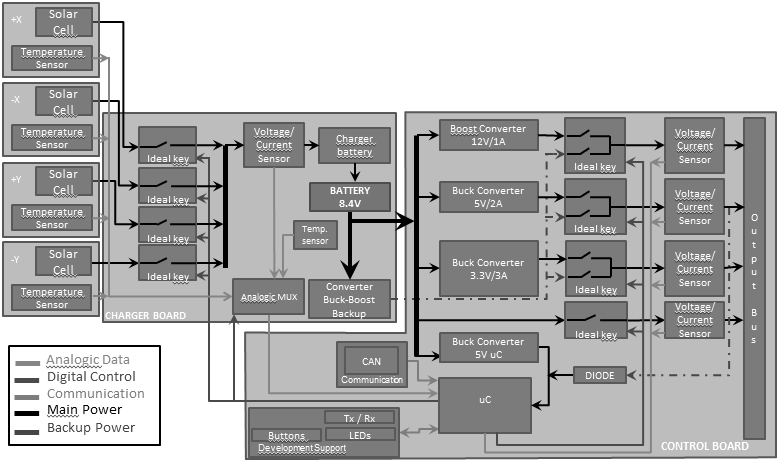
\includegraphics[width=0.8\linewidth]{./figs/diag}
		\caption{Block diagram.}
		\begin{footnotesize}
		Font: Elaborated by the authors.
		\end{footnotesize}
	\end{figure}
	
	%O projeto foi dividido em três partes de desenvolvimento, sendo elas:
	
	%\begin{itemize}
	%\item Painel solar;
	%\item Placa do carregador;
	%\item Placa de controle.
	%\end{itemize}
	
	The solar panels are responsible for capture sunlight, converting it into electricity. This electricity goes to the charger board, passes through the battery charging system and, also, by a voltage sensor and current sensor. The battery energy has two different destinies, being one of them the backup converter (that provides 3.3V, 5V and 12V, it can also provide the three voltages in the same time) and, the other one, is the control board. 
	
	In the control board there are three voltage converters of 3.3V, 5V and 12V, that are responsible for realize the supply these voltages to the output bus, where, also, is possible have the battery voltage. 
	
	In this same board is allocated a microcontroller that is powered independently, because of its dedicated converter.  However, if this converter shows any failure, the output bus can provide the 5V for keep the microcontroller working. Between the converters and the output bus, there are smart keys of low losses that make a comparative between the voltages from main converters with the backup converter and send one of them in the output. The circuit of the backup converter was projected to provide a value slightly lower than the main converters, in this way the smart keys, by default, always enable the main converters.
	
	Still on the control board, there is a microcontroller to realize the telemetry of the system and communicating via the CAN protocol, with the DPU. In case of any failure with this microcontroller, the system keeps working, losing only the communication and monitoring of sensors.
	
\section{Hardware development}
\label{Hardware development}	

	The hardware development was divided in three parts.

\subsection{\textbf{Solar panel}}
\label{Solar panel}

	For the development of solar panel, had been used solar cells of triple-junction of the model TrisolX Solar Wings, which has a efficiently approximately 28.0\%. Was realized a arrangement with four solar cells in series, managing to provide a voltage of 9.32V. Were implemented, in parallel, six sets, totaling 24 solar cells. Bypass diodes were used to avoid damages and power losses system.\cite{TrisolX}
		
\subsection{\textbf{Charger board}}
\label{Charger board}

	Here are allocated the charging battery system and the backup converter, that supply energy to output bus, in case it happens any failure in the main system. Besides having a analogic multiplex that performs the reads from temperature sensors of the solar cells according the panel desired by microcontroller.%\cite{1941}

\subsection{\textbf{Control board}}
\label{Control board}

	The control board is responsible for three main converters, smart keys of low losses and voltage and current sensors, besides the microcontroller that performs all system monitoring.%\cite{3488}\cite{563200}\cite{4412}\cite{18f}
	
	\begin{figure}[th]
  	\centering
  	  \begin{minipage}[b]{0.3\textwidth}
		\label{control}
		\centering
		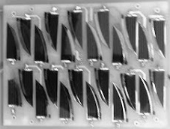
\includegraphics[width=0.6\linewidth]{./figs/cells}
	    \caption{Solar panel.}
	    
	    \begin{footnotesize}
		Font: Picture taken by the authors.
		\end{footnotesize}
	  \end{minipage}
	  \hfill
	  \begin{minipage}[b]{0.3\textwidth}
		\label{control}
		\centering
		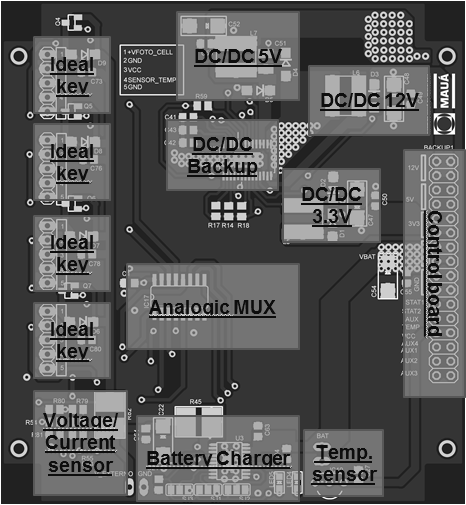
\includegraphics[width=0.7\linewidth]{./figs/charger}
	    \caption{Charger board.}
	    
	    \begin{footnotesize}
		Font: Elaborated by the authors.
		\end{footnotesize}
	  \end{minipage}
	  \hfill
	  \begin{minipage}[b]{0.3\textwidth}
		\label{charger}
		\centering
		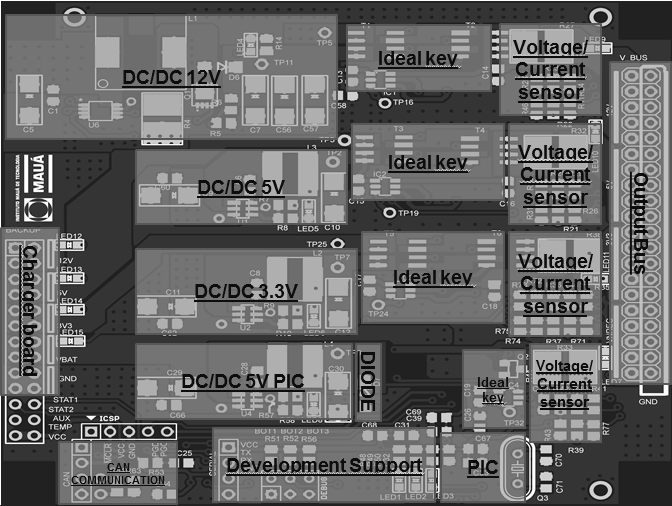
\includegraphics[width=0.6\linewidth]{./figs/control}
	    \caption{Control board, top vision.}
	    
	    \begin{footnotesize}
		Font: Elaborated by the authors.
		\end{footnotesize}
	  \end{minipage}
	\end{figure}
	
\section{Software development}
\label{Software development}

	A simple software for to run the EPS telemetry was developed, and can be seen in a simplified manner.
	
	\begin{figure}[th]
		\label{flow}
		\centering
		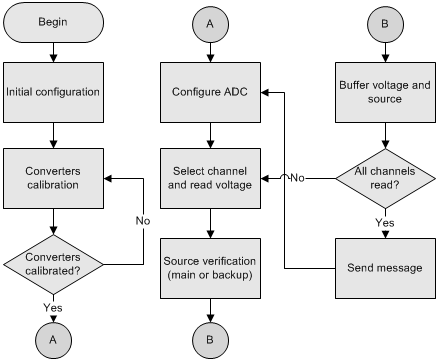
\includegraphics[width=0.3\linewidth]{./figs/fluxo2}
		\caption{Software flowchart}
	
		\begin{footnotesize}
		Font: Elaborated by the authors.
		\end{footnotesize}
	\end{figure}

	The calibration of the system is done in seven steps: the microcontroller forces the smart key to provides the voltage from the main converter, reads the value and stores into memory, then the microcontroller forces the smart key to supply the voltage from the backup converter, reads the value and compares with the main converter if there is a small difference, if the condition is satisfied it stores the value and does the same cycle for the others voltages. After that, the software gets in the main loop.

\section{Conclusion}
\label{Conclusion}

	 The solution implemented for improve the lifespan of Electrical Power System, using a backup source shows itself quite effective, the switching between the main source and backup source, with the use of ideal keys, showed itself quite functional, because has low losses and do not causes disturbances in the payload during the switching, that keeps working normally. Redundancies worked as designed by the group, so, if the main converter decrease its voltage to the point of getting the low voltage provided by the backup converter, this takes its place and begins, immediately, to provide the energy in the output bus, without the load feel switching between sources. This occurs individually for each converter or, even to all together, and does not impair the power supply to the other subsystems of the CubeSat.

%Os tópicos que se destacaram no desenvolvimento do projeto foram:
	
%	\begin{itemize}
%		\item Alta eficiência atingida com conversores de baixo custo;
%		\item Fontes de redundância de alta eficiência;
%		\item Chaveamento instantâneo entre fontes;
%		\item Utiliza\c{c}\~{a}o de componentes de f\'{a}cil acesso;
%		\item Otimiza\c{c}\~{a}o da \'{a}rea \'{u}til do \textit{CubeSat};
%		\item Desenvolvimento de \textit{software} supervisório;
%		\item Desenvolvimento de um simulador de falhas.
%	\end{itemize}


%% The Appendices part is started with the command \appendix;
%% appendix sections are then done as normal sections
%% \appendix

%% \section{}
%% \label{}

%% If you have bibdatabase file and want bibtex to generate the
%% bibitems, please use
%%
\section[References]{References}
\bibliographystyle{elsarticle-num} 
\bibliography{Article}

%% else use the following coding to input the bibitems directly in the
%% TeX file.

%\begin{thebibliography}{00}

%% \bibitem[Author(year)]{label}
%% Text of bibliographic item

%\bibitem[MEHRPARVAR, A. and PIGNATELLI, D.(2014)]{CubeSat Design Specification}

%\end{thebibliography}
\end{document}

\endinput
%%
%% End of file `elsarticle-template-harv.tex'.
